\documentclass[titlepage]{article}

\usepackage[hidelinks]{hyperref}
\usepackage[table]{xcolor}
\usepackage[english]{babel}
\usepackage{tabularx}
\usepackage[toc,page]{appendix}
\setcounter{secnumdepth}{5}
\usepackage{tikz}
\usepackage{enumitem}
\usepackage{pdfpages}
\usepackage{graphicx}
\usepackage{indentfirst} 

%
\usetikzlibrary{arrows, trees, positioning, fit, calc, shadows.blur, shapes.symbols}

\usepackage[top=1.5in, bottom=1.5in, left=2in, right=2in]{geometry}

\def\getfirstword#1{%
    \begingroup
    \edef\@tempa{#1\space}%
    \expandafter\endgroup
    \expandafter\readwords\@tempa\relax
}
\def\readwords#1 #2\relax{%
      \doword{#1}%  #1 = substr, #2 = rest of string
}
\def\doword#1{#1}
\def\endtestwords{}

\newcommand{\myparagraph}[1]{\paragraph{#1}\mbox{}\\}

\addtolength{\oddsidemargin}{-.875in}
\addtolength{\evensidemargin}{-.875in}
\addtolength{\textwidth}{1.75in}

\def \TACS {Track and Control System}

\begin{document}

\title{
\textbf{
Object Design Description}
\protect\\
for the
\protect\\
\textbf{
Track and Control System}
\protect\\
{\small Version 1.0}}

\author{Robert Moss, Aaron Periera, Matthew Shrago}
\maketitle

\newpage
\tableofcontents{} 
\newpage

\section{Introduction}

\subsection{Object Design Trade-offs}

\subsubsection{Buy vs. Build}

\item The decision to Buy vs Build can be made by:
\begin{itemize}	 	 	
  	\item If it is possible for the software to be built within a reasonable time frame using little resources, it is better to build than buy.  	
	\end{itemize}
	

\subsubsection{Space vs. Speed}

\item In the Track and Control System, space is not a major priority. With only settings and some other menial data being kept, speed is the most crucial; as a fluid motion experience is what it is striving for. 

\subsubsection{Delivery Time vs. Functionality}
\item If the development of TACS is behind schedule, the more in-depth functionalities can be sacrificed at little expense to the overall project.

\subsubsection{Delivery Time vs. Quality}
\item If testing runs behind schedule, the software can still be released and updates can be released to fix bugs at a later date.

\subsubsection{Files vs. Databases}
\item Files would not be as beneficial as a database because the data for TACS is not voluminous. A database would provide a sufficient structure to organize users and their settings. In using a file, users can theoretically edit and thus corrupt the file and the data inside. An "off site" database would be more secure and less likely to be modified.

\subsection{Interface Documentation Guidelines}
Classes
\begin{itemize}
\item Class names should be in Pascal Case.
\item i.e.: MoveWindow
\end{itemize}
Constants
\begin{itemize}
\item All constants should be entirely in Upper Case.
\item i.e.: RESOLUTION
\end{itemize}
Identifiers
\begin{itemize}
\item Identifier names should be in Camel Case.
\item i.e.: xPosition, yPosition, userSpeed
\end{itemize}
Local Variables
\begin{itemize}
\item Variables should be all lowercase, less than 8 characters long.
\item i.e.: speed
\end{itemize}
\subsection{Definitions, Acronyms, and Abbreviations}
\begin{itemize}
	\item Application Specific Definitions
	\begin{itemize}
		\item TACS - Track and Control System
		\item TM - Tracking Module
		\begin{itemize}
			\item OT - Object Tracker
			\item FRT - Facial Recognition Tracker
		\end{itemize}
		\item WCM - Windows Control Module
		\begin{itemize}
			\item WGO - Windows Grid Organizer
			\item WP - Windows Perspective
		\end{itemize}
		\item SM - Settings Module
	\end{itemize}
	\item Industry Definitions
	\begin{itemize}
		\item SRS - Software Requirements Specification
		\item OpenCV - Open Computer Vision: An open source library for object tracking via the camera.
		\item SQLite - A lightweight, low maintenance, self contained local database.
		\item DB - Database
		\item RGB - Red, Green, Blue color values.
		\item HSV - Hue, Saturation, Value.
		\item API - Application Programming Interface
		\item C++ - An object oriented programming language.
		\item GUI - Graphical User Interface
		\item QT - An API for building GUIs
	\end{itemize}
\end{itemize}


\section{Packages}

\subsection{Package Diagram}

\subsection{Package Definition}
\item This software only has one package. This package is going to contain 1 main class and 8 subclasses.


\section{Class Interface}

\subsection{Class Diagram}
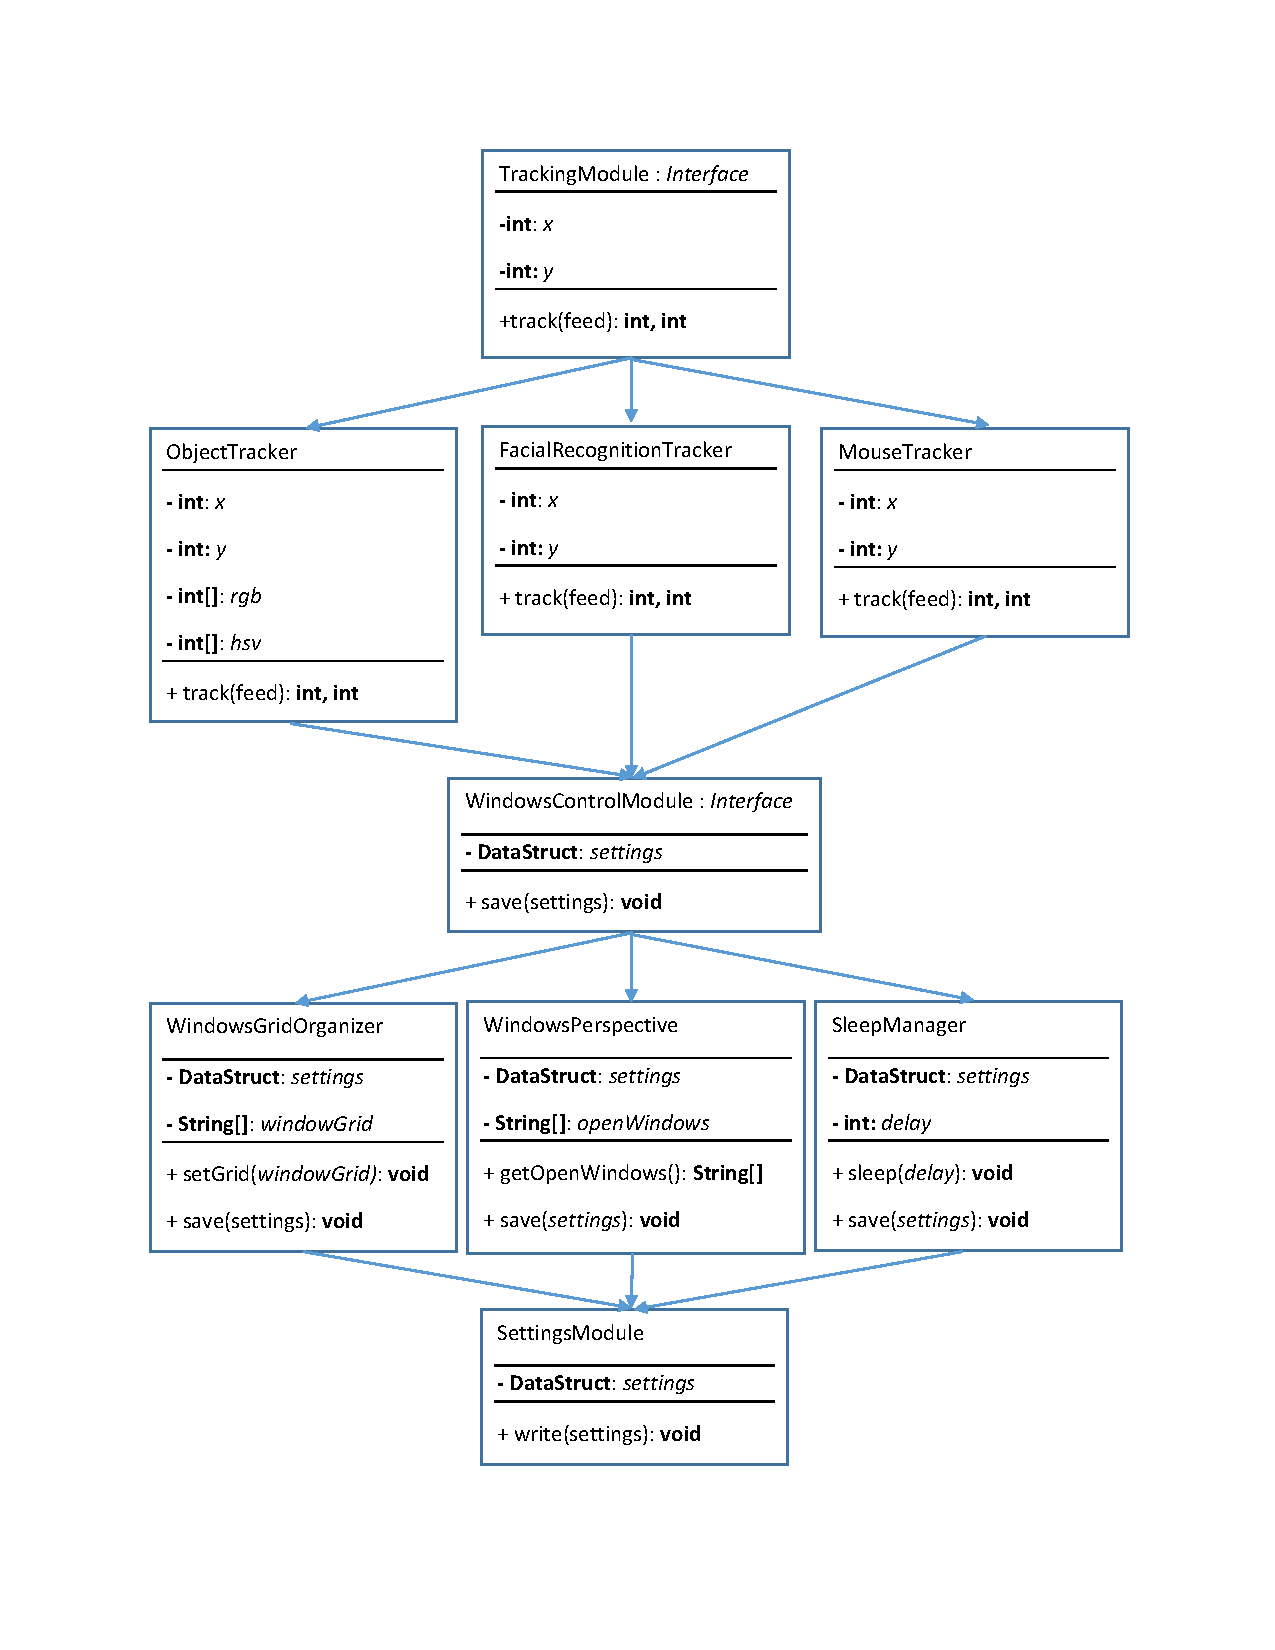
\includepdf[scale=0.75,pagecommand=\subsection{Decomposition Description}]{decomposition_description.pdf}

\subsection{Class Definition}
\item 


\end{document}